\chapter{Implementation}
\label{chp:Implementation} 

\section{Introduction}

\section{Architecture}

\section{Planner}

\begin{comment}
- Automated Planning and Scheduling
-- Offline planning: Each car has the whole map, paths can be found prior to execution
- Highest abstraction level
- Goal: Have a path ready for the robot
- Human aspect: We always drive with intention of getting from A to B
- Figure of the planner
- Algorithm
\end{comment}

Planner is the module with the highest abstraction level in the system and its main goal is to provide the cars with some meaning when they are driving. It is responsible for planning a route similar to what humans are doing. Humans are the ones that interact and sends commands to the car. Such as turning the steering wheel, indicating a turn, acceleration etc. The normal objective for a car is to transport people from A to B. The planner takes the job of always having a route for the robot to perform. Self driving cars also have the same objective, the driver tells the car where to go and the car creates a plan for this trip from A to B. 

\noindent For this projects, the environment and world map is quite simplified. There are only straight roads with simple intersections which reduces the complexity of the planner.

% http://www.cambridge.org/no/academic/subjects/computer-science/artificial-intelligence-and-natural-language-processing/automated-planning-and-acting?format=HB&isbn=9781107037274#ItlLzJTDtjPBw6TX.97
\noindent The idea of having a planner is based upon the theory of \gls{aps}, a branch of artificial intelligence that concerns the realization of strategies or actions sequences. For this thesis one of the assumptions is that all robots have a complete internal map of the environment, this means that planning can be performed offline. A solution can be found and evaluated prior to execution. In a real world scenario, in dynamically unknown environments the strategy often needs to be revised online. 

\noindent Given a description of the possible initial states in the world, a description of the desired goals, and a description of a set of possible actions, the planning problem is to synthesize a plan that is guaranteed (when applied to any of the initial states) to generate a state which contains the desired goals - the goal state. 

\noindent The simplest possible planning problem, known as the Classical Planning Problem is determined by:
\begin{itemize}
    \item a unique known initial state
    \item durationless actions
    \item deterministic actions
    \item which can be taken only one at a time
    \item a single agent
\end{itemize}

\noindent Since the initial state is know unambiguously, and all actions are deterministic, the state of the world after any sequence of actions can be accurately predicted, and the question of observability is irrelevant for classical planning. 

\noindent Given the above peculiarities the job of the planner simplifies for this project. In order for the system to guarantee full environment exploration, only a given number of steps or commands are calculated by the planner. We can construct a finite state machine that describes the planner as seen in figure \ref{fig:planner-state-machine}

\begin{figure}[H]
\centering
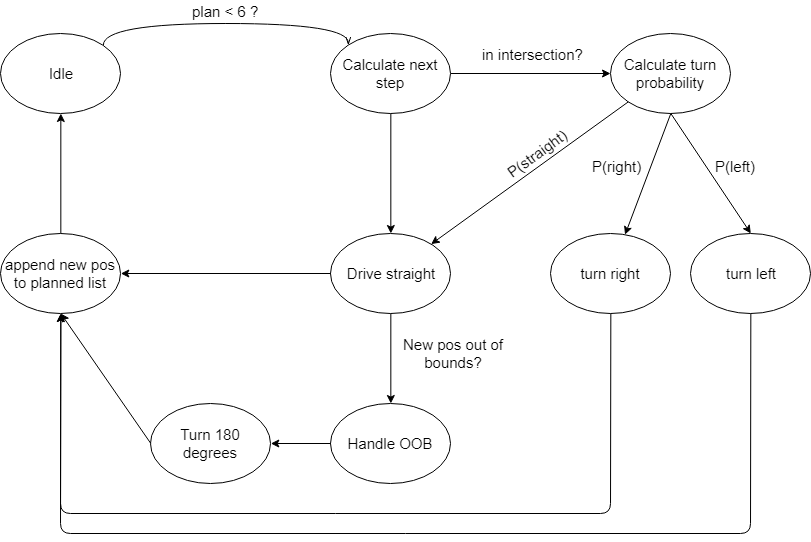
\includegraphics[width=10cm]{figs/Planner-State-Machine.png}
\caption{Planner Finite State Machine}
\label{fig:planner-state-machine}
\end{figure}

\noindent The basic operation of the planner is shown in algorithm \ref{algo:planner} in a simplified manner. The full implementation of the planner module is found in appendix X. 

\begin{algorithm}[ht]
    \caption{Basic operation for the planner module}
    \label{algo:planner}
    \begin{algorithmic}
    \While {thread is active}
        \If {$queue\_length < max\_plan\_size:$}
            \If {current location not in intersection}
                \State Add drive straight to plan
            \Else
                \State $probability = random\_probability$
                \If {$probability$ < probability of turning left}
                    \State Add turn left to plan
                \ElsIf {$probability$ < probability of turning right}
                    \State Add turn right to plan
                \Else
                    \State Drive straight
                \EndIf
            \EndIf
        \EndIf
    \EndWhile
    \end{algorithmic}
\end{algorithm}

\noindent The planner module is instantiated/initiated by the car module. Before any movement takes place the planner creates a list of 6 commands which serves as the path/plan for the robot to perform. Each time the robot is to perform a move the first command in the planner list is removed and its appropriate action is calculated based on the command. As depicted in figure \ref{fig:planner-state-machine} there are four possible actions created by the planner: drive straight, turn left, turn right and turn 180\textdegree. These commands are interpreted and consumed by the car module described in section \ref{sec:car-module}.

\section{Network}
One central aspect in order to have a working testbed is the network. In this thesis the network topology and the network module together serves as the replacement for \gls{vanet} and \gls{dsrc}. MENTION WLAN. The following subsections describe the network topology (VANET) and the onboard network module (DSRC) that provides communication. 

Raspberry Pi 3 comes with an onboard wireless interface which will serve as the \gls{dsrc} device for the robots

\subsection{Network Topology}
Raspberry Pi 3 comes with an onboard wireless interface that is used to send and receive packets in this project. Preferably, the setup of this interface should utilize the ad-hoc functionality provided by 802.11n. Due to problems of making this functionality work as expected, the ad-hoc functionality has been disabled in order to have a reliable system. 

In order for this communication to work, some configuration needs to be done on the Raspberry Pi. This is done by editing the network interface file located at $/etc/network/interfaces$. Figure \ref{fig:network-settings} displays the network configuration settings used on all Raspberry Pis in this thesis.

\begin{figure}
    \centering
    \begin{verbatim}
        auto wlan0
        iface wlan0 inet static
            address 192.168.1.1 # This address has to be unique
            netmask 255.255.255.0
            wireless-channel 1
            wireless-essid its_testbed
            wireless-mode ad-hoc
    \end{verbatim}
    \caption{\label{fig:network-settings}Network settings on Raspberry Pi}
\end{figure}

When configuring all devices in our testbed with the same settings, assigning each Raspberry Pi with a unique static IP-address, er can communicate on a peer-to-peer basis or \gls{v2v} in an ad-hoc manner. Notably, this enables the devices to communicate with every device in its vicinity. Figure \ref{fig:raspi-ad-hoc} shows the topology of the ad-hoc network in this project.

\begin{figure}
\centering
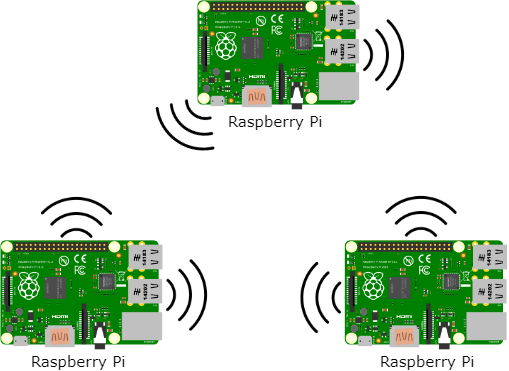
\includegraphics[width=10cm]{figs/raspi-ad-hoc.png}
\caption{Ad hoc network with Raspberry Pi 3 devices}
\label{fig:raspi-ad-hoc}
\end{figure}

\subsection{Network Module}
The network module is the module responsible for crafting, sending and receiving packets to and from other robots. For this project this module acts as the DSRC device or Onboard Unit (OU) of the car. This module is separated into two logical parts: one for sending messages and one for receiving messages, where they provide different functionality to the system. 

The concepts of \gls{vanet} and \gls{vtl} requires the use of broadcast messages in the network in order to exchange beacons (as described in...). There is also a need to separate the types of messages sent. In this projects there are two available message types: one for periodically sending beacons and one that is application specific. Since this testbed is to be a general purpose testbed for \gls{its} applications and implementation of application specific messages needs to be developed to fit the \gls{its} application being tested. In this project, an example implementation has been done for a centralized regular traffic light and a decentralized implementation of the \gls{vtl} algorithm as described in (A distributed Algorithm for VTL with IEEE 802.11p). The code for these implementations can be found in appendix X and Y. 

To handle this, the Python socket module is used. With this, one can bind a socket to an IP-address and port for sending and receiving packets over the network. In this setup User Datagram Protocol (UDP) is used for sending messages. Another option is to use the TCP protocol but this requires more overhead in the system. There are no guarantee that a UDP packet will reach its destination, which is the same for the current solutions for VANET/DSRC. To make a socket able to broadcast messages to all devices within its vicinity, the socket has to be tied up to the network broadcast address. In this network setup, the broadcast address is $192.168.1.255$. Upon receiving messages from the network, a server socket listening to messages sent to its IP-address and port, is established.

Figure x is a sequence diagram explaining how a broadcast message is sent through the ad-hoc network and received at all connected nodes. Raspberry Pi A is the sender of the message to the broadcast address. A message sent to this address will be delivered to all connected nodes in the range of the source. For the receivers - Raspberry Pi B and C - the message seems to come directly from Raspberry Pi A. 

\begin{figure}
\centering
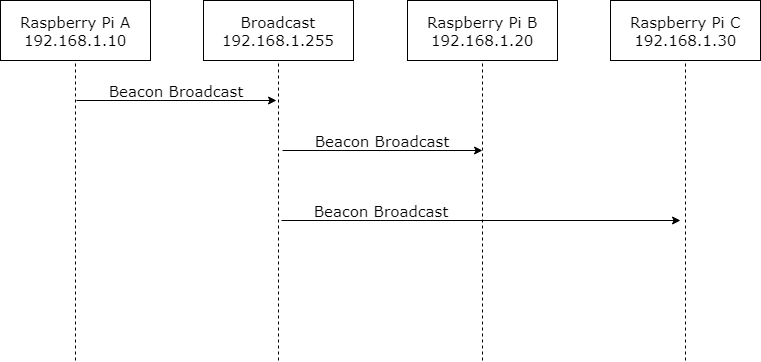
\includegraphics[width=12cm]{figs/Broadcast-Message.png}
\caption{Sequence diagram showing the flow of a broadcast message}
\label{fig:broadcast-message}
\end{figure}

\begin{figure}
\centering
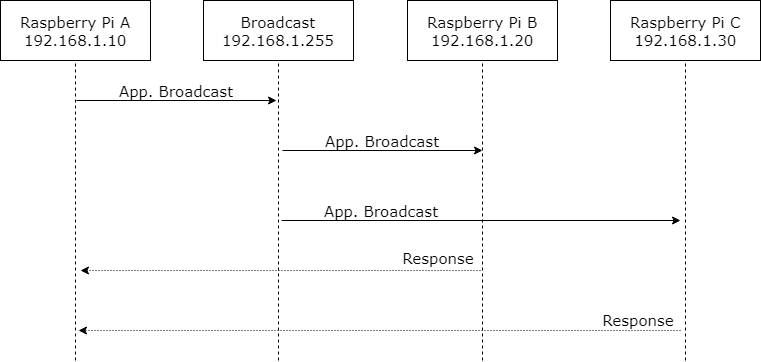
\includegraphics[width=12cm]{figs/App-Specific-Message.png}
\caption{Sequence diagram showing the flow of a application specific message with reply}
\label{fig:app-message}
\end{figure}

\begin{comment}
- VANET / DSRC
- Send / Receive
- Beacons and application specific messages
- Broadcast
\end{comment}

\section{Location}

\subsection{Environment}

\subsection{Lane Detection}

\section{Environment}

\section{Motor Control}

\section{Car}\label{sec:car-module}

\section{Data Flow}

\section{Challenges}